\chapter{Delegating Quantum Computations}



In this lecture we give a general introduction to the problem of delegating quantum computation, and then present a specific protocol due to Fitzsimons and Morimae that we will build on in the following lectures. Most of the material in the lecture is standard and may be skipped by some readers, who may nevertheless wish to briefly read over the description of the Fitzsimons-Morimae protocol in Section~\ref{sec:fm-protocol} to make sure they are comfortable with the notation introduced for it.\footnote{Some of the material for this lecture is taken from an overview of Mahadev's result written for a mathematical audience and published in the Bulletin of the AMS~\cite{vidick2020verifying}. Some of it is reproduced from lecture notes prepared for a winter school at UCSD:~\url{http://cseweb.ucsd.edu/~slovett/workshops/quantum-computation-2018/}.} 

\section{Problem statement}
\label{sec:delegation-definitions}

\subsection{Quantum circuits and the class BQP}

For us, a quantum circuit $\mC$ is specified by an integer $n$ and an ordered sequence of elements of the form $(G,i,j)$ where $G \in \{H,CNOT, T\}$ and $i,j\in\{1,\ldots,n\}$. Letting 
\begin{equation}\label{eq:gateset}
 H = \frac{1}{\sqrt{2}} \begin{pmatrix} 1 & 1 \\ 1 & -1 \end{pmatrix}\;,\qquad CNOT = \begin{pmatrix} 1 & 0 & 0 & 0 \\ 0 & 1 & 0 & 0 \\ 0 & 0 & 0 & 1 \\ 0 & 0 & 1 & 0 \end{pmatrix}\;,\qquad T = \begin{pmatrix} 1 & 0 \\ 0 & e^{i\pi/4}\end{pmatrix}\;,
\end{equation}
the circuit $\mC = ((G_1,i_1,j_1),\ldots,(G_T,i_k,j_k))$ represents the unitary $U$ on $(\C^2)^{\otimes n}$ obtained as $U = U_T \cdots U_1$ where for all $t\in\{1,\ldots,T\}$, $U_t$ acts as the unitary associated with $G_t$ in~\eqref{eq:gateset} on qubits $i_t$ and $j_t$ and as identity on the other qubits. (In case $G_t\in\{H,T\}$ it is required that $i_t=j_t$.) The Solovay-Kitaev theorem shows that any $n$-qubit unitary can be arbitrary well-approximated, in operator norm, by the unitary derived from a circuit; however, the size of the circuit may (in fact, must) in general grow exponentially fast with $n$. Those unitaries that can be represented by small circuits are called ``efficient''. 

Given a quantum circuit $\mC$ acting on $n$ qubits and $x\in\{0,1\}^m$ for some $m\leq n$ we say that ``$\mC$ accepts input $x$ with probability $p$'' if the probability of obtaining the outcome $1$ after a measurement in the computational basis of the first qubit of the $n$-qubit state obtained by applying the unitary $\mC$ to the input state $\ket{x}\ket{0^{n-m}}$ is $p$.

\begin{definition}
We say that a promise language $L=(L_{yes},L_{no})$ is in $\BQP$ if there exists a family of polynomial-time generated quantum circuits $\{\mC_n\}_{n\in\N}$ such that for all integer $n$ and $x\in\{0,1\}^n$,\footnote{Note that in general, $\mC_n$ may act on $\poly(n)$ qubits, the first $n$ of which are by convention destined to receive the input $x$ and the first of which also serves as output qubit.}
\begin{itemize}
\item (Completeness:) If $x\in L_{yes}$ then $\mC_n$ accepts $x$ with probability at least $\frac{2}{3}$;
\item (Soundness:) If $x\in L_{no}$ then $\mC_n$ accepts $x$ with probability at most~$\frac{1}{3}$.
\end{itemize}
\end{definition}

Note the requirement that the family $\{\mC_n\}$ is polynomial-time generated. This means that there exists a classical Turing Machine that on input $1^n$ runs in time $\poly(n)$ and returns a description of $\mC_n$ as a sequence of gates taken from a fixed universal set---here we use~\eqref{eq:gateset}, but the specific choice will not matter for us. 

The definition of BQP sets arbitrary values $2/3$ and $1/3$ for the completeness and soundness parameters. Error amplification works just as for the case of BPP, by repeating the circuit sequentially. This requires intermediate measurements, but it is not hard to show that these can be postponed till the end of the computation by the use of ancilla qubits and CNOT gates.
 As a result, any choice of $a,b$ such that $a-b > \poly^{-1}(n)$ gives the same definition: for any such $a,b$, and for any fixed polynomial $q$,  $\BQP(a,b)=\BQP=\BQP(1-2^{-q},2^{-q})$. 


\begin{exercise}\label{ex:pp}
Show that BQP is included in PP, the class of languages for which there exists a probabilistic Turing machine that accepts YES inputs with probability $>1/2$, and rejects NO inputs with probability $>1/2$. (Hint: first show inclusion in PSPACE by giving space-efficient implementations of basic linear algebra operations. Inclusion in PP follows from similar arguments, but is a bit more delicate.)
\end{exercise}

The class $\PP$ lies outside of the polynomial hierarchy. The most commonly-held belief is that the intersection of $\BQP$ and $\PH$ is non-trivial: it is neither $\BPP$, nor $\PH$ itself. Recently Raz and Tal~\cite{raz2019oracle} showed that an oracle problem introduced by Aaronson~\cite{aaronson2010bqp} is in $\BQP$ but not in $\PH$. 

We end this section by defining a family of complexity classes associated with interactive proof systems. 

\begin{definition}[Adapted from~\cite{aharonov2017quantum}]
Given complexity classes $\mP$ and $\mQ$, $\IP[\mP,\mQ]$ is the class of (promise) languages $L$ such that there is a polynomial-time Turing machine $M$ that on input $1^n$ returns the description of classical circuits for the verifier $V_n$ in an interactive protocol with a prover $P$ such that 
\begin{itemize}
\item (Completeness:) There is a family of provers $\{P_n\}_{n\in \N}$ that lie in the class $\mP$ such that for all $x\in L$ the interaction of $V_{|x|}$ and $P_{|x|}$ on common input $x$ accepts with probability at least $\frac{2}{3}$.
\item (Soundness:) For any family of provers $\{P_n\}_{n\in \N}$ that lie in the class $\mQ$, for all $x\in L_{no}$ the interaction of $V_{|x|}$ and $P_{|x|}$ on common input $x$ accepts with probability at most $\frac{1}{3}$.
\end{itemize}
When the classes $\mP$ and $\mQ$ coincide we simply write $\IP[\mP]$ for $\IP[\mP,\mP]$. We use the standard notation $\IP = \IP[ \BPP, \ALL]$ with $\ALL$ the class of all languages (i.e.\ soundness is proves without any restriction on the prover). 
\end{definition}

The definition is slightly informal, because for some classes $\mP$ it may not be clear what it means for the prover to lie in $\mP$. For us the meaning will always be clear from context, as $\mP$ and $\mQ$ will always be either $\BPP$, $\BQP$ or $\ALL$. 


\subsection{Delegating quantum computations}

The fact that $\BQP$ is not (believed to be) in $\NP$ implies that in general we do not expect there to exist classically verifiable proofs for the correctness of an arbitrary quantum computation. This poses a challenge: as we see quantum computers emerging, how will we test their predictions? This is a practical problem --- will anyone trust the ``quantum cloud'' --- but also a philosophical one --- is quantum mechanics a testable theory? (For more on this, see~\cite{aharonov2013quantum}.)

Not all is lost. What we \emph{do} know is that $\BQP$ is included in $\PSPACE$, the class of languages that can be decided using polynomial space (and arbitrary time); in fact Exercise~\ref{ex:pp} asked you to show a stronger statement. And even though it is not a trivial result, it is known that $\PSPACE = \IP$. 
So all languages in $\BQP$ have \emph{classical} interactive proofs, with an efficient classical verifier! Unfortunately there is a major caveat to this observation. The proof that $\PSPACE$ is in $\IP$ is based on the classical SUM-CHECK protocol, which in general requires the server to execute $\PSPACE$-complete computations (essentially, the server has to compute exponentially large sums in order to determine answers that will satisfy the client). (For an exposition of the proof we refer to the book~\cite{arora2009computational}.)


 So, even though a protocol exists, it is unknown if there is such a protocol in which a honest server is only required to have the power of $\BQP$. Today this is a major open question: 

\begin{oq}
Is $\BQP \subseteq \IP[\BQP,\ALL]$? In words, do all languages in $\BQP$ have single-server interactive proofs in which the client has the power of $\BPP$ and for which completeness holds with a $\BQP$ server and soundness holds against any server? 
\end{oq}

There are some  partial impossibility results~\cite{aaronson2017implausibility} on this question, as well as possibility results where completeness holds for provers that require more power than $\BQP$ but not necessarily the entire power of $\PSPACE$; see e.g.~\cite{aharonov2017quantum}. If, however, one allows slightly more power to the verifier then there are scenario in which the question is known to have a positive answer: 
\begin{enumerate}
\item The client has access to a limited quantum computer, such as the ability to prepare single qubits in arbitrary states and send them to the server, or receive single qubits from the server and make simple measurements on them;
\item The client is allowed to interact with multiple quantum servers sharing entanglement.
\end{enumerate}

The question as formulated above asks for \emph{verifiable} delegation: given a quantum circuit (deciding some $\BQP$ language $L$), is there a protocol that allows a classical client to extract the outcome of the circuit from a $\BQP$ server, in a way that any cheating server, attempting to convince the client of the wrong outcome, will be detected?  A second desirable property of a delegation protocol is \emph{blindness}: while the client would like to learn the valid outcome of her circuit, she might not want to disclose the particular circuit or input she is interested in to the server. This is a distinct property from verifiability; in particular, one may ask for blindness in the ``honest-but-curious'' model, where verifiability is trivial. The following definition introduces these properties slightly more formally. 


\begin{definition}[Delegated computation]
In the task of delegated computation, a client (sometimes called the \emph{verifier}) has an input $(x,\mC)$, where $x$ is a classical string and $\mC$ the classical description of a quantum circuit. The client has a multiple-round interaction with a quantum server (sometimes also called \emph{server}). At the end of the interaction, Alice either returns a classical output $y$, or she aborts. A protocol for delegated computation is called:
\begin{itemize}
\item \emph{Correct} if whenever both the client and the server follow the protocol, with high probability Alice accepts (she does not abort) and $y=\mC(x)$. (This property is sometimes called \emph{completeness}.) 
\item \emph{Verifiable} if for any server deviating from the protocol, the client either aborts or returns $y=\mC(x)$.  (This property is analogous to what we have been calling \emph{soudness}.) 
\item \emph{Blind} if for any server deviating from the protocol, at the end of the protocol the server has no information at all about the client's input $(x,\mC)$. 
\end{itemize}
\end{definition}

The definition remains rather informal. For example, how should we formalize the ``information'' that the server has at the end of the computation? This can be rather delicate, especially once one starts taking into account a small chance $\eps$ of deviation from the perfect properties. A precise definition satisfying all the desired properties (universal composability in particular) would take us too far. Such a definition was given using the framework of \emph{abstract cryptography} in~\cite{dunjko2014composable}. 

The informal definition will be sufficient for our purposes. Note that in spite of being rather similar neither of the properties of verifiability or blindness is known to directly implies the other. In practice verifiability often follows from blindness by arguing, using ``traps'', that if a protocol is already blind then the server's trustworthiness can be tested by making it run ``dummy'' computations for which Alice already knows the output, without the server being able to distinguish whether it is asked to do a real or dummy computation. We will see an example of this technique later on. 

\begin{oq}
Is there a general transformation from any protocol satisfying blindness, to a protocol satisfying both verifiability and blindness? See~\cite{kashefi2017quantum} for a possible approach. 
\end{oq}

\begin{remark}
The problem of delegating computation is interesting even for classical computation. In this case the client herself could directly execute the classical circuit $\mC$. But it makes sense to be even more demanding, and seek protocols where the client is super-efficient: the best we could hope for is a client that runs in time \emph{linear} in the input length, and independent of the size of the circuit. In addition, we would like the overhead for the server to be as small as possible, so that the honest behavior requires a server effort of the same order as the size of the circuit, $|\mC|$. This kind of interactive proofs are called \emph{doubly efficient} interactive proofs~\cite{goldwasser2008delegating}. The paper~\cite{reingold2016constant} shows how to achieve such proofs with client runtime that is linear in the input length, polynomial in the space required by $\mC$, and polylogarithmic in $|\mC|$. If one is willing to make computational assumptions (essentially, subexponential LWE) then even more efficient delegation is possible~\cite{kalai2014delegate}, with client runtime that is linear in the input size and poly-logarithmic in $|\mC|$. 

These results usually do not put emphasis on the requirement of blindness: they focus on verifiability alone. One reason for this is that blindness is ``trivially solved'' by employing homomorphic encryption~\cite{gentry2009fully}. This, however, requires computational assumptions, and induces significant computational overhead. 
\end{remark}


\section{The Fitzsimons-Morimae protocol}
\label{sec:fm}

We describe the receive-and-measure protocol from~\cite{morimae2016post}, as it will form the basis for the Mahadev protocol. 


\subsection{The circuit-to-Hamiltonian reduction}
\label{sec:certificates-q}

The Cook-Levin theorem showing NP-completeness of the $3$SAT problem is based on what could be called a ``circuit-to-formula'' reduction: given a classical circuit, the computation performed by the circuit on some input is represented as a ``tableau'' such that the property of being a valid tableau can be encoded in a formula whose variables represent the state of any given wire in the circuit and whose constraints enforce correct propagation of the gates of the circuit. 

\begin{figure}[htb!]
\centering%
%\hfill
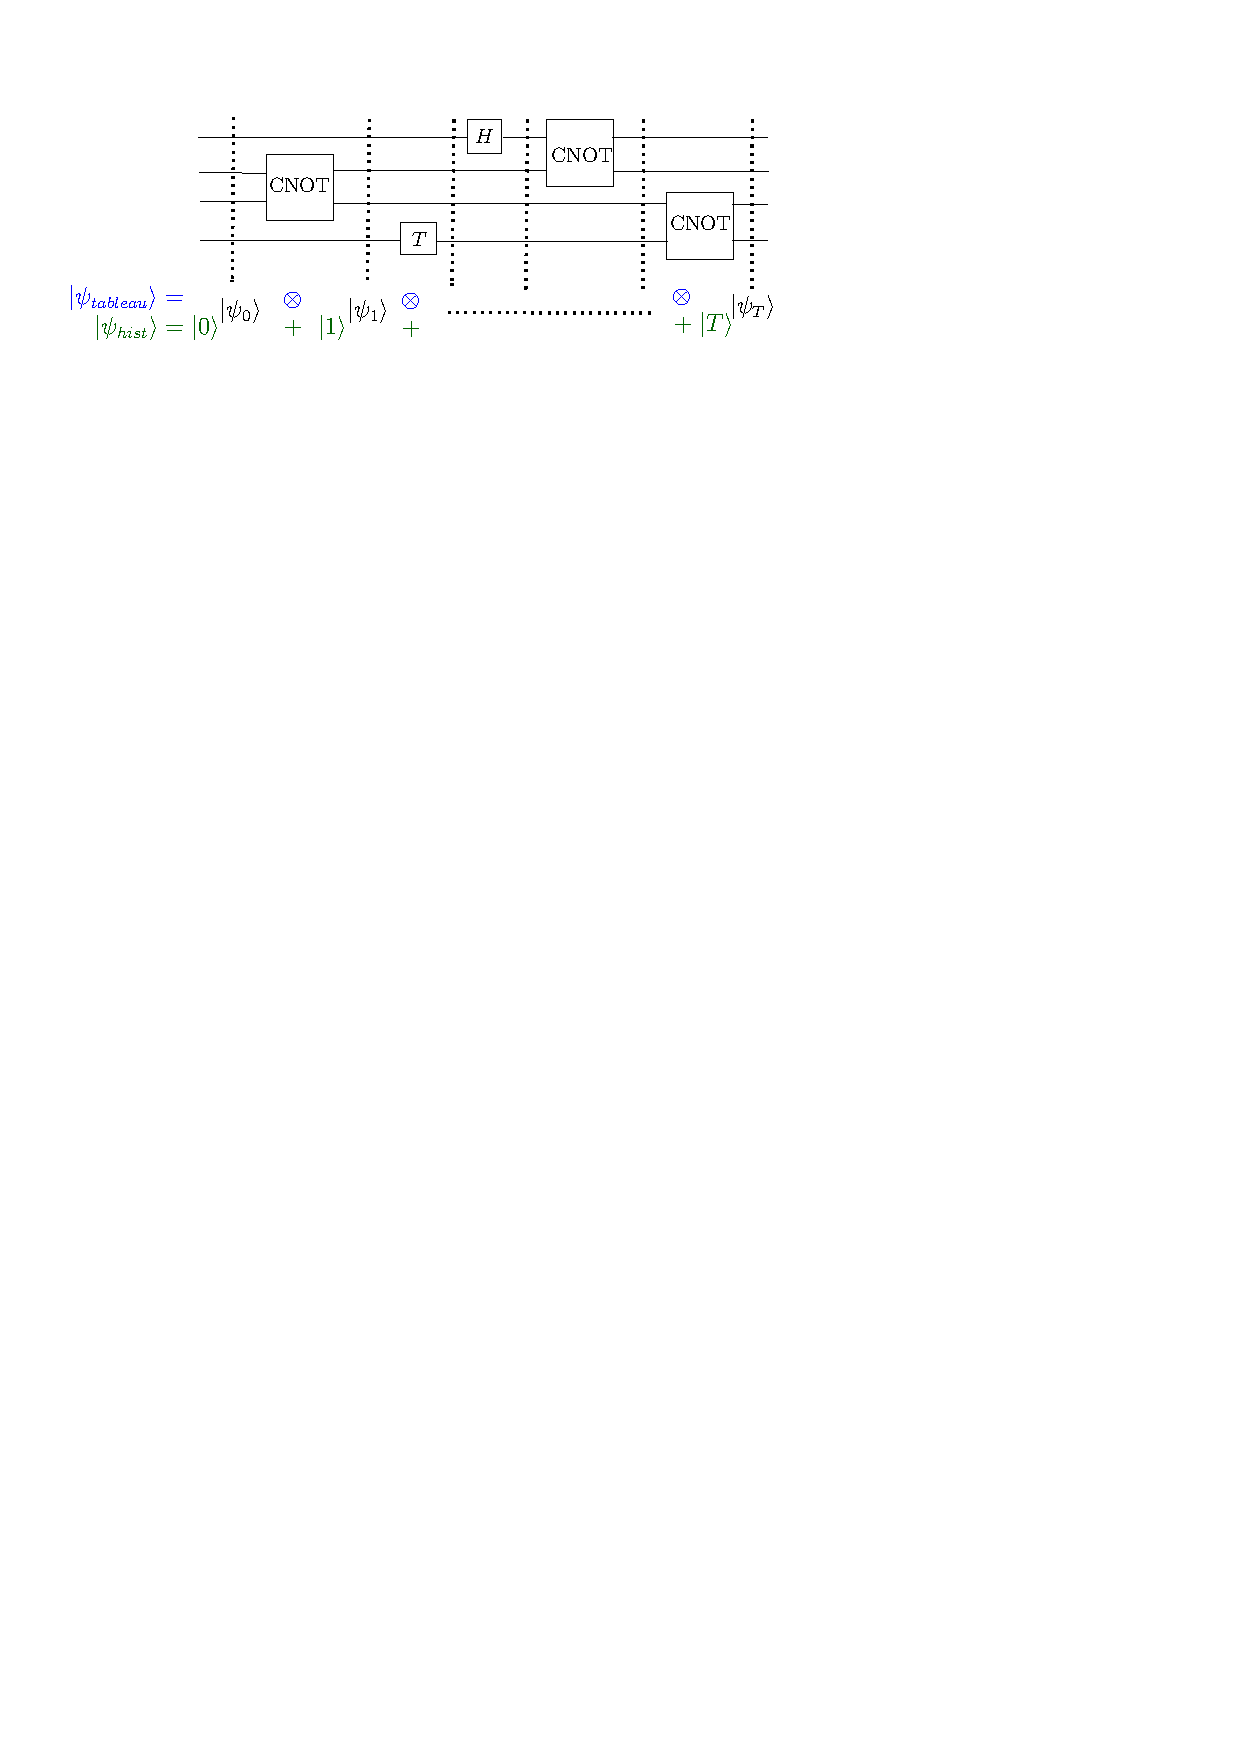
\includegraphics[scale=1, angle = 0]{qtableau.pdf}
%\hfill
\caption{Two different ways to create a tableau from a quantum circuit. The state $\ket{\psi_{tableau}}$ is the tensor product of the state of the circuit at each time step. The state $\ket{\psi_{hist}}$ is their superposition, indexed by a clock register that goes from $\ket{0}$ to $\ket{T}$.}
\label{fig:q-tableau}
\end{figure}


For quantum circuits the idea of a tableau of the computation is less straightforward. The most direct analogue is to consider the juxtaposition of the quantum state of a $T$-gate circuit at each step of the computation, i.e. the tensor product $\ket{\psi_0}\otimes \cdots\otimes \ket{\psi_T}$ of the states $\ket{\psi_i}$ obtained by executing the circuit from scratch and stopping after $i$ gates have been applied. While this is a well-defined $n(T+1)$-qubit quantum state (see Figure~\ref{fig:q-tableau}) the property of being a valid ``quantum tableau'' cannot be enforced using \emph{local} constraints! The reason is subtle, and has to do with the possible presence of entanglement at intermediate steps of the computation. Indeed, there are quantum states that are very different, in the sense that they are perfectly distinguishable by some \emph{global} observable, yet cannot be distinguished at all by any \emph{local} observable, that would act on at most, say, half the qubits. An example is given by the two $n$-qubit ``cat'' (named after the homonymous animal) states
\[ \ket{\psi_{\pm}} = \frac{1}{\sqrt{2}} \big( \ket{0\cdots 0} \pm \ket{1\cdots 1} \big)\;.\]
The two states $\ket{\psi_+}$ and $\ket{\psi_-}$ are easily seen to be orthogonal, so that they can be perfectly distinguished by a measurement. But it is an exercise to verify that for any observable that acts on at most $(n-1)$ of the $n$ qubits, both states give exactly the same expectation value. (Informally, this is because any measurement on a strict subset of the qubits of the state necessarily destroys the coherence; the only relevant information, the $\pm$ sign, is encoded ``globally'' and cannot be accessed locally.)
Note that this is a uniquely quantum phenomenon: if two classical strings of bits have each of their bits equal, one pair at a time, then the strings are ``globally'' identical. Not so for quantum states.

So na\"ive tableaus will not do. In the late 1990s Alexei Kitaev introduced a very powerful idea that provides a solution. Kitaev's idea is to replace the juxtaposition of snapshot states by their \emph{superposition} (see Figure~\ref{fig:q-tableau}). A special ancilla system, called the ``clock'', is introduced to index different elements of the superposition. Thus, instead of defining a tableau as $\ket{\psi_0} \cdots \ket{\psi_T}$, Kitaev considers the state
\begin{equation}\label{eq:h-state}
 \ket{\psi_{hist}}\,=\,\frac{1}{\sqrt{T+1}} \sum_{t=0}^T \ket{t}\ket{\psi_t}\;.
\end{equation}
Note that this takes less qubits to store, but this is not the important point. 
 Kitaev showed that, assuming the clock register is encoded in unary, it is possible to check the correct propagation of every step of the circuit directly on this superposition by only applying local observables: there is a set of observables $H_{in}$ that checks that $\ket{\psi_0}$ has the right format; a set of observables $H_{prop}$ that checks propagation of the circuit, and an observable $H_{out}$ that checks that the output qubit of the circuit is in the right state. (In addition, there is a term $H_{clock}$ that checks that the clock register is well-formed, i.e. contains the representation of an integer in unary. This can be done locally by penalizing configurations of the form ``$\cdots 10\cdots$''.) The key point that makes this possible is that, while equality of quantum states cannot be decided locally when the states are juxtaposed, it becomes possible when they are given in superposition. As an exercise, we can verify that a measurement of the first qubit of the state
\[ \ket{\psi_{SWAP}} \,=\, \frac{1}{\sqrt{2}}\big( \ket{0} \ket{\psi_0} + \ket{1}\ket{\psi_1}\big)\]
in the Hadamard basis $\{ \ket{+},\ket{-}\}$ returns the first outcome with probability exactly $\frac{1}{2}(1+|\bra{\psi_0}\psi_1\rangle|^2)$. 
With more work, replacing the use of gadgets in the classical Cook-Levin reduction by techniques from perturbation theory, it is possible to write the resulting observables as a linear combination of local terms that all take a particularly simple form. 
The result is the following theorem from~\cite{cubitt2016complexity}.

\begin{theorem}\label{thm:kitaev}
For any integer $n\geq 1$ there are $n'=\poly(n)$, $a=a(n)$ and $\delta \geq 1/\poly(n)$ such that the following holds. 
Given a $T$-gate quantum circuit $\mC = ((G_1,i_1,j_1),\ldots,(G_T,i_T,j_T))$ acting on $n$ qubits, such that $T=\poly(n)$, and an input $x$ for the circuit, there exist efficiently computable real weights $\{J_{ij},\, i,j\in\{1,\ldots,n'\}\}$ such that $|J_{ij}|\leq 1$ for all $i,j$ and moreover if
\begin{equation}\label{eq:lh-comp}
H_\mC \,=\, - \sum_{i,j}\; \frac{J_{ij}}{2}\,\big(\sigma_{X,i} \sigma_{X,j} + \sigma_{Z,i} \sigma_{Z,j}\big)\;,
\end{equation}
where $\sigma_{X,i}$ and $\sigma_{Z,j}$ denote single-qubit Pauli $X$ and $Z$ operators acting on the $i$-th and $j$-th qubit respectively, 
then:
\begin{itemize}
\item (Completeness) If the circuit $\mC$ accepts its input $x$ with probability at least $2/3$, then the smallest eigenvalue of $H_\mC$ is at most a;
\item (Soundness) If the circuit $\mC$ accepts its input $x$ with probability at most $1/3$, then the smallest eigenvalue of $H_\mC$ is at least $a + \delta$.
\end{itemize} 
\end{theorem}

\begin{remark}
It is possible to modify Theorem~\ref{thm:kitaev} so that the completeness and soundness statements specify that ``if there exists a state $\ket{\phi}$ such that $\mC$ accepts on input $(x,\ket{\phi})$ with probability at least $2/3$...'' and ``if there does not exist a state $\ket{\phi}$ such that $\mC$ accepts on input $(x,\ket{\phi})$ with probability greater than $1/3$...'' respectively. Thus, Theorem~\ref{thm:kitaev} can be adapted to show that the problem of estimating the minimal energy of a Hamiltonian of the form~\eqref{eq:lh-comp} is a QMA-complete problem. 
\end{remark}


Theorem~\ref{thm:kitaev} provides us with a roadmap for the verification of quantum circuits: it is sufficient to verify the \emph{existence} of a quantum state that yields certain statistics, when some of its qubits are measured in the computational ($\sigma_Z$ observable) or Hadamard ($\sigma_X$ observable) basis. The reason this can be considered progress is that we no longer need to check the time evolution of a quantum state under a quantum cicuit; it is sufficient to collect measurement statistics and estimate the ``energy'' $\bra{\psi}H\ket{\psi}$.  In particular, the theorem readily leads to a verification protocol in a model where the prover has a full quantum computer, and the verifier only has a limited quantum device --- namely, a one-qubit memory, together with the ability to measure the qubit using either the $\sigma_X$ or $\sigma_Z$ observables. 


\subsection{The protocol}
\label{sec:fm-protocol}

Such a verification protocol was introduced by Fitzsimons and Morimae and refined in a paper with Hadju\v{s}ek. The protocol is summarized in Figure~\ref{fig:fhm-protocol}. In the protocol, the prover is required to prepare a smallest eigenstate of the Hamiltonian $H_\mC$ given in~\eqref{eq:lh-comp}. While it may not be immediately obvious at the level of our description, it is possible to prepare such a ``history state''~\eqref{eq:h-state} by executing a quantum circuit that is only mildly more complex than the original circuit $\mC$. 

\begin{figure}[htbp]
\rule[1ex]{16.5cm}{0.5pt}\\
Let $\mC$ be a quantum circuit provided as input, and $H_\mC$ the $n$-qubit Hamiltonian obtained from $\mC$ as in~\eqref{eq:lh-comp}. 
\begin{enumerate}
\item The verifier initializes a counter $\gamma$ to $0$. She executes the following interaction with the prover independently $N=\frac{C}{\delta^2} {n' \choose 2}^2 \ln(1/\eps)$ times, where $C$ is a large enough universal constant:
\begin{enumerate}
\item The prover creates an eigenstate $\ket{\psi}$ of $H$ with smallest eigenvalue. 
\item The prover sends the qubits of $\ket{\psi}$ one by one to the verifier.
\item The verifier selects a measurement $W\in\{X,Z\}$ uniformly at random, and measures each qubit in the associated basis upon reception. Let $b_{W,i}\in\{-1,1\}$ be the outcome for the $i$-th qubit. 
\item The verifier selects $i\neq j \in \{1,\ldots,n'\}$ uniformly at random. She updates her counter $\gamma \leftarrow \gamma - J_{ij} b_{W,i} b_{W,j}$.
\end{enumerate}
\item If $\frac{\gamma}{N }{n' \choose 2} \leq a + \delta/2$ the verifier accepts the interaction. Otherwise, she rejects. 
\end{enumerate}
\rule[1ex]{16.5cm}{0.5pt}
\caption{The Fitzsimons-Hadju\v{c}ek-Morimae verification protocol, parametrized by a quantum circuit $\mC$ and an accuracy parameter $\eps>0$.}
\label{fig:fhm-protocol}
\end{figure}

We note that in the protocol, the verifier measures the qubits in a randomly chosen basis, and then selects a single pair $(i,j)$ such that $J_{ij}\neq 0$ uniformly at random to update her counter. One could imagine small optimizations where e.g.\ a maximum matching of such pairs is measured at each step. Such optimizations only bring marginal improvements in efficiency of the protocol; moreover they complicate the extension to a classical verifier that we will see later. For this reason, we prefer to keep the simplest expression possible for the protocol. 


\begin{theorem}\label{thm:fm}
Let $\mC$ be a quantum circuit and $H_\mC$ the Hamiltonian associated to it as in~\eqref{eq:lh-comp}. Let $x$ be an input to the circuit $\mC$ and $\eps>0$ a parameter for the protocol. Then the following hold:
\begin{itemize}
\item (Completeness:) If $\mC$ accepts $x$ with probability at least $2/3$, then there is a QPT prover that is accepted with probability at least $1-\eps$
\item (Soundness:) If $\mC$ accepts $x$ with probability at most $1/3$, then any prover is accepted with probability at most $\eps$. 
\end{itemize}
\end{theorem}

Note that in the theorem, the soundness statement does not place any computational assumption on the prover. 

\begin{proof}
The key calculation that underlies the proof is the following. 

\begin{claim}\label{claim:fm-1}
Let $\rho$ be the density matrix that represents the mixture over the $N$ $n'$-qubit states sent by the prover in the protocol (in general these states may be entangled). Then the expectation of $\gamma/N$ is exactly
\begin{equation}\label{eq:fm-eq-1}
\Es{} \Big[ \frac{\gamma}{N} \Big] \,=\, -\frac{1}{ {n' \choose 2}} \,\sum_{i\neq j}\, \frac{J_{ij}}{2} \,\Tr\big(\big(\sigma_X^i \sigma_X^j + \sigma_Z^i \sigma_Z^j\big)\rho\big)\,=\, \frac{1}{ {n' \choose 2}}\, \Tr\big(H\rho\big)\;.
\end{equation}
Moreover, for $N$ chosen as in the protocol for a large enough choice of the constant $C$ it holds that
\begin{equation}\label{eq:fm-eq-2}
\Pr\Big( \Big|\frac{\gamma}{N} {n'\choose 2} - \Tr\big(H\rho\big)\Big|> \frac{\delta}{2} \Big) \,\leq \,\eps\;.
\end{equation}
\end{claim} 

\begin{proof}
For $t\in\{1,\ldots,n\}$ let $G_t$ denote the product of the two outcomes $b_{W,i}$ and $b_{W,j}$ obtained by the verifier at step (c) of the protocol, where $W$, $i$ and $j$ are as sampled at step (d). Then the random variables $G_t \in \{-1,1\}$ are i.i.d. such that for each $t$, $\Es{}[G_t]= \Tr(\sigma_W^i \sigma_W^j \rho)$, with $W$, $i$ and $j$ are the values sampled in step $t$. Since $\gamma = - \sum_t J_{ij} G_t$, averaging over those choices gives~\eqref{eq:fm-eq-1}. Using $|J_{ij}|\leq 1$, by Hoeffding's inequality for any $s>0$
\[ \Pr\big( \big|\gamma - \Es{}[\gamma]\big| > s \big) \,\leq \, e^{-\frac{2  s^2 }{ 4N}}\;.\]
By choosing $N$ sufficiently large with respect to ${n' \choose 2}^2\delta^{-2}\ln(1/\eps)$ we get~\eqref{eq:fm-eq-2}.
\end{proof}

Based on Claim~\ref{claim:fm-1} the proof of Theorem~\ref{thm:fm} follows rather directly. For the completeness, we take $\rho = \proj{\psi}$ such that $\bra{\psi} H \ket{\psi} \leq a$, whose existence is guaranteed by the completeness case of Theorem~\ref{thm:kitaev}. As noted above, this $\rho$ can be prepared efficiently by a QPT prover. Using~\eqref{eq:fm-eq-2} it follows that this prover is accepted with probability at least $1-\eps$. For the soundness, $\rho$ is arbitrary. Using the soundness case of Theorem~\ref{thm:kitaev} it must be that $\Tr(H\rho) \geq a+\delta$, so that the conclusion follows again from~\eqref{eq:fm-eq-2}. 
\end{proof}




Even though the verifier's ``quantumness'' in this protocol is limited --- she only needs to hold one qubit at a time --- this capability is crucial for the analysis, as it is used to guarantee the ``existence'' of the state that is being measured: it allows us to meaningfully talk about ``the state $\rho$ whose first qubit is the first qubit received by the verifier; whose second qubit is the second qubit received by the verifier; etc.''. These qubits are distinct, because the verifier has seen and then discarded them (it would be a different matter if they were returned to the prover). In particular, the fact that a one-qubit computer can be trivially simulated on a classical piece of paper is immaterial to the argument.

With a classical verifier things become substantially more delicate. How can we verify the existence of an $n$-qubit state with certain properties, while having only access to classical data about the state, data that, for all we know a priori, could have been generated by a simple --- classical --- laptop? To achieve this we need to find a way for the verifier to establish that the prover holds an $n$-qubit state, without ever having the ability to directly probe even a single qubit of that state. In the previous lecture we saw a means to achieve this for a single qubit based on the computational hardness of certain functions called ``claw-free''. In the next lecture we extend that method to introduce a protocol by which the prover can certify the existence of any single-qubit state that is a low-energy eigenstate of a single-qubit Hamiltonian. In the last lecture we combine this extension with the Fizsimons-Morimae protocol to obtain a protocol for delegating quantum computations with a classical client. 
